%%%%%%%%%%%%%%%%%%%%%%%%%%%%%%%%%%%%%%%%%%%%%%%%
%% Compile the master file!
%% 		Slides: Antonio Machicao y Priemer
%% 		Course: GK Linguistik
%%%%%%%%%%%%%%%%%%%%%%%%%%%%%%%%%%%%%%%%%%%%%%%%


%%%%%%%%%%%%%%%%%%%%%%%%%%%%%%%%%%%%%%%%%%%%%%%%%%%%
%%%             Metadata                         
%%%%%%%%%%%%%%%%%%%%%%%%%%%%%%%%%%%%%%%%%%%%%%%%%%%%      

\title{Grundkurs Linguistik}

\subtitle{Semantik II \& Pragmatik I}

\author[A. Machicao y Priemer]{
	{\small Antonio Machicao y Priemer}
	\\
	{\footnotesize \url{http://www.linguistik.hu-berlin.de/staff/amyp}}
	%	\\
	%	\href{mailto:mapriema@hu-berlin.de}{mapriema@hu-berlin.de}}
}

\institute{Institut für deutsche Sprache und Linguistik}

\date{ }

%\publishers{\textbf{6. linguistischer Methodenworkshop \\ Humboldt-Universität zu Berlin}}

%\hyphenation{nobreak}


%%%%%%%%%%%%%%%%%%%%%%%%%%%%%%%%%%%%%%%%%%%%%%%%%%%%
%%%             Preamble's End                   
%%%%%%%%%%%%%%%%%%%%%%%%%%%%%%%%%%%%%%%%%%%%%%%%%%%%      


%%%%%%%%%%%%%%%%%%%%%%%%%    
\huberlintitlepage[22pt]
\iftoggle{toc}{
\frame{
\begin{multicols}{2}
	\frametitle{Inhaltsverzeichnis}\tableofcontents
	%[pausesections]
\end{multicols}
}
}


%%%%%%%%%%%%%%%%%%%%%%%%%%%%%%%%%%
%%%%%%%%%%%%%%%%%%%%%%%%%%%%%%%%%%
%%%%%LITERATURE:

\nocite{Brandt&Co06a} 
\nocite{Glueck05a} 
\nocite{Grewendorf&Co91a} 
\nocite{Luedeling2009a} 

%% Allgemein
\nocite{Glueck&Roedel16a}
\nocite{Luedeling2009a}
\nocite{Meibauer&Co07a} 
\nocite{Repp&Co15a} 

%% Morphologie
%\nocite{Eisenberg04}

%% Syntax
%\nocite{Adger04a}
%\nocite{Altmann&Hofmann08a} % Satztypen & Satzmodi
%\nocite{Altmann93a} % Satztypen & Satzmodi
%\nocite{Brandt&Co06a} 
%\nocite{Fanselow&Sascha87a}
%\nocite{Fanselow&Sascha93a}
%\nocite{Fries&MyP16b} % Akzeptabilität
%\nocite{Fries16a} % Grammatikalität
%\nocite{Fries&MyP16d} % Kompetenz vs Performanz
%\nocite{Fries&MyP16c} % GG
%\nocite{Fries&MyP16a} % X-Bar-Theorie
%\nocite{Fries16e} % Satztyp
%\nocite{Fries16d} % Satzmodus 
\nocite{Grewendorf&Co91a} 
%\nocite{MyP17b} % Kerngrammatik
%\nocite{MyP18a} % Konstituententest
%\nocite{MyP18b} % Kopf
%\nocite{MyP18c} % Phrase
%\nocite{MyP18s} % Funktionale Kategorie
%\nocite{MyP18t} % Argumentstruktur
%\nocite{MuellerS13f} 
%\nocite{MuellerS15b}
%\nocite{Stechow&Sternefeld88a}
%\nocite{Sternefeld06a}
%\nocite{Sternefeld06b}
%\nocite{Woellstein10a} % Topologisches Feldermodell

%% Semantik & Pragmatik
\nocite{Loebner15a} %% Semantics
\nocite{Loebner15b} %% Semantics
\nocite{Lohnstein11} %% Semantics
%\nocite{MyP16a} %% Bikonditional
\nocite{Partee&Co93a} %% Semantics
\nocite{ZimmermannT&Sternefeld13a} %% Semantics


%%%%%%%%%%%%%%%%%%%%%%%%%%%%%%%%%%%
\section{Pragmatik}
%%%%%%%%%%%%%%%%%%%%%%%%%%%%%%%%%%

\begin{frame}
\frametitle{Begleitlektüre}

	\begin{itemize}
	\item AM S.~107--116
	\item \citet{Meibauer&Co07a}: Kapitel 6 (S.~210--240)
\end{itemize}

\end{frame}


%%%%%%%%%%%%%%%%%%%%%%%%%%%%%%%%%%%
%%%%%%%%%%%%%%%%%%%%%%%%%%%%%%%%%%%
%
\subsection{Einführung}

%% MyP: Contents
\iftoggle{sectoc}{
	\frame{
		%\begin{multicols}{2}
		\frametitle{~}
		\tableofcontents[currentsubsection,subsubsectionstyle=hide]
		%\end{multicols}
	}
}
%%%%%%%%%%%%%%%%%%%%%%%%%%%%%%%%%%%%%

\begin{frame}
\frametitle{Einführung}

\begin{itemize}
	\item Pragmatik \ras jüngste sprachwissenschaftliche Disziplin
	\item Schnittstellen zur Philosophie, Soziologie, Psychologie
	\item Gegenstand \ras \textbf{Gebrauch} sprachlicher Ausdrücke in einer bestimmten Situation (Kontext)
	\item[]
	\item Semantik \vs Pragmatik (grob):
	
	\begin{itemize}
		\item Semantik:\\
kontextunabhängige (und durch Wahrheitsbedingungen erfassbare) Bedeutung
		\item Pragmatik: \\
kontextabhängige  (und durch Wahrheitsbedingungen nicht erfassbare) Bedeutung
	\end{itemize}
	
\end{itemize}

\end{frame}


%%%%%%%%%%%%%%%%%%%%%%%%%%%%%%%%%%%%%%%

\begin{frame}
\frametitle{Einführung}

\begin{itemize}
	\item Semantik \ras Bedeutung aus Wörtern + Strukturen
	\item[]
	\item Pragmatik \ras kontextuell relevante Interpretation
	
	\begin{itemize}
		\item Ich habe zwei Flaschen Wein.
		
		\begin{itemize}
			\item Semantik: Der Sprecher besitzt zwei Flaschen, die mit Wein gefüllt sind.
			\item Pragmatik: Der Sprecher besitzt nicht mehr als zwei Flaschen. (Nutzung: Zollerklärung, Angebot, Mitteilung, \dots)
		\end{itemize}
	\end{itemize}
\end{itemize}

\end{frame}


%%%%%%%%%%%%%%%%%%%%%%%%%%%%%%%%%%%%%%%
%%%%%%%%%%%%%%%%%%%%%%%%%%%%%%%%%%%%%%
%
\subsection{Kontext}
%
%%%%%%%%%%%%%%%%%%%%%%%%%%%%%%%%%%%%%%%%
%% MyP: Contents
\iftoggle{sectoc}{
	\frame{
		%\begin{multicols}{2}
		\frametitle{~}
		\tableofcontents[currentsubsection,subsubsectionstyle=hide]
		%\end{multicols}
	}
}
%%%%%%%%%%%%%%%%%%%%%%%%%%%%%%%%%%%%%

\begin{frame}
\frametitle{Kontext}

\begin{itemize}
	\item Kontextuell relevante Aspekte von Bedeutung:
	
\vspace{5mm}
	
	\begin{itemize}
		\item \textbf{Äu\ss{}erungssituation} \\
Zeitpunkt, Sprecher, Hörer, \dots
		\item []
		\item \textbf{Sprachlicher Kontext}\\
Vorhergehende Äu\ss{}erungen, Diskurs-Thema, \dots
		\item[]
		\item \textbf{Informationeller Kontext} \\
Was wei\ss{} der Sprecher, was nimmt der Sprecher über den Hörer an, Weltwissen, \dots
		\item []
		\item \textbf{Intentionaler Kontext} \\
Was sind die Ziele/""Wünsche/""Pläne des Sprechers?
	\end{itemize}
	
\end{itemize}

\end{frame}


%%%%%%%%%%%%%%%%%%%%%%%%%%%%%%%%%%%%%%%%%%%%%
%%%%%%%%%%%%%%%%%%%%%%%%%%%%%%%%%%%%%%%%%%%%%%
%
\subsubsection{Deixis}
%
%%%%%%%%%%%%%%%%%%%%%%%%%%%%%%%%%%%%%%%%%%%%
%\iftoggle{sectoc}{
%\frame{
%\frametitle{~}
%	\tableofcontents[currentsubsection,subsubsectionstyle=hide]
%}
%}
%%%%%%%%%%%%%%%%%%%%%%%%%%%%%%%%%%%%%%%%%%%%

\begin{frame}
\frametitle{Deixis}

\begin{itemize}
	\item Deixis \ras Vorgang des Zeigens
	\item[]
	\item \textbf{Deiktische} (oder indexikalische) \textbf{Ausdrücke} \ras Sprachliche Ausdrücke, die sich auf die Aspekte der Äu\ss{}erungssituation beziehen (Person-, Raum- und Zeitstruktur)
	\item[]
	\item Referenz \ras Aspekte der Äu\ss{}erungssituation
	\item[]
	\item Referenz von deiktischen Ausdrücken anders als bei referierenden Ausdrücken
\end{itemize}

\end{frame}


%%%%%%%%%%%%%%%%%%%%%%%%%%%%%%%%%%%%%%%

\begin{frame}
\frametitle{Deixis}

\begin{itemize}
	\item \textbf{Personaldeixis} 
	
	\begin{itemize}
		\item Aktuelle Gesprächsrollen
		\item Sprecher/Adressat: ich, du, wir, \dots
	\end{itemize}
	
	\item \textbf{Sozialdeixis}
	
	\begin{itemize}
		\item Distanzform für Adressaten: Sie (\vs du)
	\end{itemize}
	
	\item \textbf{Objektdeixis}
	
	\begin{itemize}
		\item Situativ-deiktisch verwendete Pronomina
		\item Referenz auf 3. Pers./Obj.: dieser, jener, der, er, \dots
	\end{itemize}
	
\end{itemize}

\end{frame}


%%%%%%%%%%%%%%%%%%%%%%%%%%%%%%%%%%%%%%%
\begin{frame}
\frametitle{Deixis}

\begin{itemize}
	\item \textbf{Lokaldeixis}
	
	\begin{itemize}
		\item Referenz auf Ort: hier, dort, \dots
	\end{itemize}
	
	\item \textbf{Temporaldeixis}
	
	\begin{itemize}
		\item Referenz auf Zeit: gestern, heute, \dots
	\end{itemize}
	
\end{itemize}

\end{frame}


%%%%%%%%%%%%%%%%%%%%%%%%%%%%%%%%%%%%%
%%%%%%%%%%%%%%%%%%%%%%%%%%%%%%%%%%%%%
%
\subsubsection{Anaphorik}
%
%%%%%%%%%%%%%%%%%%%%%%%%%%%%%%%%%%%%%%
%\iftoggle{sectoc}{
%	\begin{frame
%\frametitle{~}
%	\tableofcontents[currentsubsection,subsubsectionstyle=hide]
%}
%}
%%%%%%%%%%%%%%%%%%%%%%%%%%%%%%%%%%%%%%%

\begin{frame}
\frametitle{Anaphorik}

\begin{itemize}
	\item \textbf{Anaphorische Ausdrücke (Anapher)}\\
Sprachliche Ausdrücke, die sich auf sprachliche Einheiten im vorhergehenden sprachlichen Kontext beziehen
	\item[]
	\item Anaphorik \vs Deixis \ras Art des Kontextes
	\item[]	
	\item \textbf{Textdeixis}
	
	\eal 
	\ex Peter hat sich rasiert.
	\ex Die Hausaufgabe war so einfach, dass alle sie sehr schnell lösen konnten.
	\zl
	
\end{itemize}
	
\end{frame}


%%%%%%%%%%%%%%%%%%%%%%%%%%%%%%%%%%%%%%%

\begin{frame}
\frametitle{Anaphorik}

\begin{itemize}
	\item \textbf{Koreferenz}\\
Bezug zweier (oder mehrerer) Ausdrücke auf den gleichen Referenten in einem Text (oder Satz).
	\item[]
	\item \textbf{Antezedens} \\
Erstgenannter referentieller Ausdruck in einer anaphorischen Kette
		
		\eal 
		\ex Peter hat sich rasiert. (Syntaktische Anapher = Reflexivpron.)
		\ex Die Hausaufgabe war so einfach, dass alle sie sehr schnell lösen konnten.
		\zl
		
		\begin{itemize}
			\item Antezedens: \gqq{Peter} von \gqq{sich} und \gqq{die Hausaufgabe} von \gqq{sie}
		\end{itemize}
	
\end{itemize}

\end{frame}


%%%%%%%%%%%%%%%%%%%%%%%%%%%%%%%%%%%%%%%

\begin{frame}
\frametitle{Anaphorik}

\begin{itemize}
	\item \textbf{Anapher}
	
	\ea Wie viel an \textbf{Grice} auch immer auszusetzen ist, selbst die schärfsten Kritiker sehen \textbf{ihn} als einen der wichtigsten Pragmatiker an.
	\z
	
	\item \textbf{Katapher}
	
	\ea Wie viel an \textbf{ihm} auch immer auszusetzen ist, selbst die schärfsten Kritiker sehen \textbf{Grice} als einen der wichtigsten Pragmatiker an.
	\z
	
\end{itemize}

\end{frame}


%%%%%%%%%%%%%%%%%%%%%%%%%%%%%%%%%%%%%%%
%%%%%%%%%%%%%%%%%%%%%%%%%%%%%%%%%%%%%%
%
\subsubsection{Übung}
%
%%%%%%%%%%%%%%%%%%%%%%%%%%%%%%%%%%%%%%%%
%%%%%%%%%%%%%%%%%%%%%%%%%%%%%%%%%%%%%%%
%\iftoggle{sectoc}{
%\begin{frame
%\frametitle{~}
%	\tableofcontents[currentsubsection,subsubsectionstyle=hide]
%}
%}
%%%%%%%%%%%%%%%%%%%%%%%%%%%%%%%%%%%%%%%

\begin{frame}
\frametitle{Übung}

\begin{itemize}
	\item Markieren und bestimmen Sie die deiktischen und anaphorischen Ausdrücke.
	
	\begin{enumerate}
	\item Morgen werde ich sie besuchen, obwohl es mir zeitlich nicht passt.
	\item[]
	\item Gestern regnete es vor dem Supermarkt.
	\item[]
	\item Am 10.02.2014 hat Peter einen Sack Kartoffeln gekauft.
	\item[]
	\item Ich treffe Sie in Ihrem Büro.
	\item[]
	\item Der Dozent wei\ss{}, dass es gut für Sie ist, das zu lernen.
	\item[]
	\item Karl hat nicht hingeschaut und dann hat er mich angefahren.
	\item[]
	\item Mario hat ihn rasiert und Peter hat sich gewaschen.
	\end{enumerate}
	
\end{itemize}

\end{frame}


%%%%%%%%%%%%%%%%%%%%%%%%%%%%%%%%%%%%%%%

\iftoggle{ue-loesung}{
	
	%%%%%%%%%%%%%%%%%%%%%%%%%%%%%%%%%%
%% UE 1 - 08 Pragmatik
%%%%%%%%%%%%%%%%%%%%%%%%%%%%%%%%%%

\begin{frame}
\frametitle{Übung -- Lösung}

Markieren und bestimmen Sie die deiktischen und anaphorischen Ausdrücke.
	
	\begin{enumerate}
		\item \textbf{Morgen} (Temporaldeixis) werde \textbf{ich} (Personaldeixis) \textbf{sie} (Personaldeixis) besuchen, obwohl es \textbf{mir} (Personaldeixis) zeitlich nicht passt.
		\item[]
		\item \textbf{Gestern} (Temporaldeixis) regnete es \textbf{vor dem Supermarkt} (Lokaldeixis).
		\item[]
		\item Am 10.02.2014 hat Peter einen Sack Kartoffeln gekauft.
		\item[]
		\item \textbf{Ich} (Personaldeixis) treffe \textbf{Sie} (Sozialdeixis) in \textbf{Ihrem} (Sozialdeixis) Büro.
		\item[]
		\item Der Dozent wei\ss{}, dass es gut für \textbf{Sie} (Sozialdeixis) ist, \textbf{das} (Objektdeixis) zu lernen.
		\item[]
		\item Karl hat nicht hingeschaut und dann hat \textbf{er} (Anapher) \textbf{mich} (Personaldeixis) angefahren.
		\item[]
		\item Mario hat \textbf{ihn} (Katapher) rasiert und Peter hat \textbf{sich} (Anapher) gewaschen.
	\end{enumerate}     

\end{frame}
	
}

%%%%%%%%%%%%%%%%%%%%%%%%%%%%%%%%%%%%%%%
%%%%%%%%%%%%%%%%%%%%%%%%%%%%%%%%%%%%%%
%
\subsection{Typen von Folgerungen}
%
%%%%%%%%%%%%%%%%%%%%%%%%%%%%%%%%%%%%%%%%
%%%%%%%%%%%%%%%%%%%%%%%%%%%%%%%%%%%%%%%
%% MyP: Contents
\iftoggle{sectoc}{
	\frame{
		%\begin{multicols}{2}
		\frametitle{~}
		\tableofcontents[currentsubsection,subsubsectionstyle=hide]
		%\end{multicols}
	}
}
%%%%%%%%%%%%%%%%%%%%%%%%%%%%%%%%%%%%%%%

\begin{frame}
\frametitle{Typen von Folgerungen}

\begin{itemize}
	\item Arten von Schlüssen, die aus einer Äu\ss{}erung gezogen werden können
	\item Unterschiede: Logische Eigenschaften und Bedingungen für die Gültigkeit

\vspace{1ex}
	\item \textbf{Semantische Implikation (Entailment)}
	
	\ea Ge\ss{}ler tötete Ge\ss{}ler.\\ $|$ = Ge\ss{}ler ist gestorben.
	\z
	
	\item \textbf{Präsupposition}
	
	\ea Maria hat aufgehört zu rauchen.\\ $>>$ Maria hat geraucht.
	\z

	\item \textbf{Implikatur}
	
	\ea Ich habe zwei Kinder.\\ + $>$ Ich habe NUR zwei Kinder.
	\z

\end{itemize}

\end{frame}


%%%%%%%%%%%%%%%%%%%%%%%%%%%%%%%%%%%%%%%
%
\subsubsection{Semantische Implikation}
%
%%%%%%%%%%%%%%%%%%%%%%%%%%%%%%%%%%%%%%%
%\iftoggle{sectoc}{
%	\begin{frame
%		\frametitle{~}
%		\tableofcontents[currentsubsection,subsubsectionstyle=hide]
%	}
%}
%%%%%%%%%%%%%%%%%%%%%%%%%%%%%%%%%%%%%%%

\begin{frame}
\frametitle{Semantische Implikation}

\begin{itemize}
	\item Semantische Implikation  = Entailment ( $|$ =)
	\item []
	\item p impliziert q, gdw. in allen Welten, in denen p wahr ist, auch q wahr ist (aber nicht notwendigerweise umgekehrt).
	\item[]
	\item Logik der Teilaussagen steht in einer inhaltlichen Beziehung zueinander (anders als \textbf{materiale Implikation}).

	\eal
		\ex Die Frau wurde erstochen.
		\ex Die Frau ist tot.
	\zl

\end{itemize}

\end{frame}


%%%%%%%%%%%%%%%%%%%%%%%%%%%%%%%%%%%%%%%

\begin{frame}
\frametitle{Semantische Implikation}

\begin{itemize}
	\item p impliziert q, gdw. in allen Welten, in denen p wahr ist, auch q wahr ist (aber nicht notwendigerweise umgekehrt).
	\item[]
	\item \textbf{Gegenseitige} semantische Implikation (\ras Synonymie)
	
	\eal
		\ex Die Katze steht auf der Matte.
		\ex Die Matte liegt unter der Katze.
	\zl
	
	\item \textbf{Einseitige} semantische Implikation (\ras Hyponymie)
	
	\eal
		\ex Die Frau wurde erstochen.
		\ex Die Frau wurde umgebracht.
	\zl
	
	\begin{itemize}
		\item p impliziert/folgert semantisch/entails q:
		\item p $|$ = q
	\end{itemize}
	
\end{itemize}

\end{frame}


%%%%%%%%%%%%%%%%%%%%%%%%%%%%%%%%%%%%%%%

\begin{frame}
\frametitle{Semantische Implikation}

\begin{figure}
	\centering
	\LARGE
	
\textbf{	Der untere Satz ist eine Lüge.}

\vspace{2cm}

\textbf{Der obere Satz ist wahr.}

\end{figure}
%\begin{figure}
%\centering
%
%%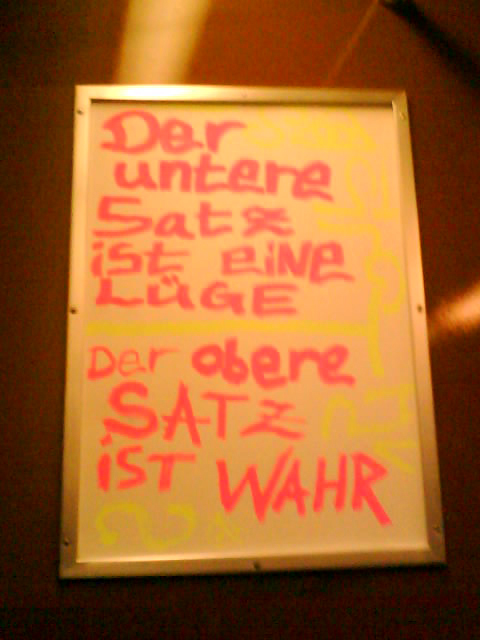
\includegraphics[scale=0.3]{material/13Pragv}
%
%\end{figure}

\end{frame}


%%%%%%%%%%%%%%%%%%%%%%%%%%%%%%%%%%%%%%%
%%%%%%%%%%%%%%%%%%%%%%%%%%%%%%%%%%%%%%%
%
\subsubsection{Präsupposition}
%
%%%%%%%%%%%%%%%%%%%%%%%%%%%%%%%%%%%%%%%
%\iftoggle{sectoc}{
%	\begin{frame
%		\frametitle{~}
%		\tableofcontents[currentsubsection,subsubsectionstyle=hide]
%	}
%}
%%%%%%%%%%%%%%%%%%%%%%%%%%%%%%%%%%%%%%%

\begin{frame}
\frametitle{Präsupposition}

\begin{itemize}
	\item Implizite Voraussetzung ($\gg$)
	\item Präsuppositionen werden nicht vom Wahrheitsgehalt eines Satzes erfasst.
	\item Präsuppositionen müssen erfüllt sein, damit der Satz einen Wahrheitswert haben kann!

\vspace{1ex}

		\ea \label{ex11} Der gegenwärtige König von Frankreich ist kahlköpfig.
		\z
		
		\begin{itemize}
			\item (\ref{ex11}) ist wahr, wenn es einen kahlköpfigen König von Frankreich gibt.
			\item (\ref{ex11}) ist falsch, wenn es keinen kahlköpfigen König von Frankreich gibt.
			\item (\ref{ex11}) kann kein Wahrheitswert zugeordnet werden, wenn \gqq{es keinen König von Frankreich gibt}.
		\end{itemize}
	
\end{itemize}

\end{frame}



%%%%%%%%%%%%%%%%%%%%%%%%%%%%%%%%%%%%%%%%%%%%%%%%%%%%%%%%%%%%%%%%

\begin{frame}
\frametitle{Präsupposition}

\begin{itemize}
	\item \textbf{Semantische} Präsupposition  (Bedingung für Wahrheit)
	
	\begin{itemize}
		\item p präsupponiert semantisch q, gdw.

		\begin{itemize}
			\item in allen Welten, in denen p wahr ist, auch q wahr ist,
			\item in allen Welten, in denen p falsch ist, q wahr ist.
		\end{itemize}

	\end{itemize}
	
\vspace{1ex}

	\item \textbf{Pragmatische} Präsupposition (Sprachgebrauch)
	
	\begin{itemize}
		\item Ein Sprecher S präsupponiert (pragmatisch) q mit der Äu\ss{}erung von p, wenn er davon ausgeht, dass q gemeinsames Sprecher-Hörer-Wissen ist.
	\end{itemize}
	
\end{itemize}

\end{frame}


%%%%%%%%%%%%%%%%%%%%%%%%%%%%%%%%%%%%%%%%%%%%%%%%%%%%%%%%%%%%%%%%%%%

\begin{frame}
\frametitle{Präsuppositionstests}

\begin{itemize}
	\item Zur Unterscheidung von Präsuppositionen und Assertionen (wahrheitsfunktionaler Gehalt einer Äu\ss{}erung)
	\item[]
	\item \textbf{Negationstest}
	
	\begin{itemize}
		\item Präsupposition bleibt erhalten (vgl. semantische Implikation)		
		
		\ea Maria hat aufgehört zu rauchen.\\ $\gg$ Maria hat geraucht.
		\z
		
		\ea Es ist nicht der Fall, dass Maria aufgehört hat zu rauchen.\\ $\gg$ Maria hat geraucht.
		\z
		
	\end{itemize}	

\end{itemize}	



\end{frame}


%%%%%%%%%%%%%%%%%%%%%%%%%%%%%%%%%%%%%%%

\begin{frame}
\frametitle{Präsuppositionstests}

\begin{itemize}
	\item \textbf{Modalisierungstest}
	
	\begin{itemize}
		\item Präsupposition bleibt erhalten (vgl. semantische Implikation)

		\ea Peters Freundin ist krank.\\ $\gg$ Peter hat eine Freundin.
		\z
		
		\ea Peters Freundin ist wahrscheinlich/vielleicht krank.\\ $\gg$ Peter hat eine Freundin.
		\z
	
	\end{itemize}
	
\end{itemize}

\end{frame}


%%%%%%%%%%%%%%%%%%%%%%%%%%%%%%%%%%%%%%%%%%%%%%%%%%%%

\begin{frame}
\frametitle{Präsuppositionstest}

\begin{itemize}
	\item \textbf{Frage- und Aufforderungstest}
	
	\begin{itemize}
		\item Präsupposition bleibt erhalten (vgl. semantische Implikation)

		\ea Peter schlägt immer noch seine Frau.\\ $\gg$ Peter hat seine Frau geschlagen.
		\z
		
		\ea Schlägt Peter immer noch seine Frau?\\ $\gg$ Peter hat seine Frau geschlagen.
		\z
		
		\ea Schlag (immer) noch deine Frau!\\ $\gg$ Peter hat seine Frau geschlagen.
		\z
		
		\end{itemize}

\end{itemize}

\end{frame}


%%%%%%%%%%%%%%%%%%%%%%%%%%%%%%%%%%%%%%% 

\begin{frame}
\frametitle{Präsuppositionstests}

\begin{itemize}
\item \textbf{Konditionalisierungstest}

\vspace{5mm}

	\begin{itemize}
		\item Präsupposition bleibt erhalten (vgl. semantische Implikation)
		
		\ea Auch Andrea studiert noch.\\
			$\gg$ Andrea studierte bisher.\\
			$\gg$ Andere studieren auch.
		\z

			\ea Wenn auch Andrea noch studiert, dann bekommt sie kein Bafög mehr. \\
			$\gg$ Andrea studierte bisher.\\
			$\gg$ Andere studieren auch.
		\z

	\end{itemize}
	
\end{itemize}

\end{frame}


%%%%%%%%%%%%%%%%%%%%%%%%%%%%%%%%%%%%%%%%%%%%%%%

\begin{frame}
\frametitle{Präsuppositionstests}

\begin{itemize}
	\item Präsuppositionen werden nicht durch Wahrheitsbedingungen erfasst.
	
	\begin{itemize}
		\item negierbar, erfragbar, modalisierbar
	\end{itemize}
	
	\item Präsupposition muss erfüllt sein, damit der Satz einen Wahrheitswert haben kann!
	
	\ea \label{ex21} Der gegenwärtige König von Frankreich ist kahlköpfig.
	\z
		
		\begin{itemize}
			\item (\ref{ex21}) ist wahr, wenn es einen König von Frankreich gibt, der kahlköpfig ist.
			\item (\ref{ex21}) ist falsch, wenn es einen König von Frankreich gibt, der aber nicht kahlköpfig ist.
			\item (\ref{ex21}) kann kein Wahrheitswert zugeordnet werden, wenn \gqq{es keinen König von Frankreich gibt}!
		\end{itemize}

\end{itemize}

\end{frame}


%%%%%%%%%%%%%%%%%%%%%%%%%%%%%%%%%%%%%%%%%%%%%%%

\begin{frame}
\frametitle{Präsuppositionsauslöser}

\begin{itemize}
	\item \textbf{Eigennamen}
	
	\ea Kepler starb im Elend. \\ $\gg$ Es gibt ein Individuum namens Kepler.
	\z

	\item \textbf{Definite DPs}
	
	\ea Der König von Frankreich ist kahlköpfig.\\ 
	$\gg$ Es gibt (genau) einen König von Frankreich.
	\z
	
	\item \textbf{Verben der Zustandsveränderung}

	\ea Es hat aufgehört zu regnen.\\
			$\gg$ Es hat (mal) geregnet.
	\z

\end{itemize}

\end{frame}


%%%%%%%%%%%%%%%%%%%%%%%%%%%%%%%%%%%%%%%%%%%%%%%

\begin{frame}
\frametitle{Präsuppositionsauslöser}

\begin{itemize}
	\item \textbf{Temporalsätze}
	
	\ea Bevor Sie die Klausur geschrieben haben, hatten Sie Ihre Hausaufgaben zurück bekommen.\\
		$\gg$ Sie haben die Klausur geschrieben.
	\z

	\item \textbf{Temporaladverbien}
	
	\ea Peter ist noch krank.\\
		$\gg$ Peter war krank.
	\z
	
	\item \textbf{Faktive Verben}
	
		\ea Sie wissen, dass Sie abgehört werden.\\
		$\gg$ Sie werden abgehört.
		\z
	
\end{itemize}

\end{frame}


%%%%%%%%%%%%%%%%%%%%%%%%%%%%%%%%%%%%%%%%%%%%%%%

\begin{frame}
\frametitle{Präsuppositionsaufhebung}

\begin{itemize}
	\item Aufhebbarkeit durch
	
\vspace{5mm}

	\begin{itemize}
		\item unmittelbaren Kontext:
		
		\ea Maria hat Peter nicht verlassen.\\
			$\gg$ Maria war mit Peter zusammen.
		\z
		
		\item Maria hat Peter nicht verlassen, denn sie waren nie zusammen.
		
\vspace{5mm}

		\item Diskurskontext:
		
		\ea Peter bedauert, den Wagen gekauft zu haben.\\ 
			$\gg$ Peter hat den Wagen gekauft.
		\z
			
		\item Peter wird nicht bedauern (müssen), den Wagen gekauft zu haben \\(auch möglich, wenn Peter den Wagen nicht gekauft hat).
				
	\end{itemize}
					
\end{itemize}


\end{frame}


%%%%%%%%%%%%%%%%%%%%%%%%%%%%%%%%%%%%%%%%%%%%%%%
%
\subsubsection{Implikatur}
%
%%%%%%%%%%%%%%%%%%%%%%%%%%%%%%%%%%%%%%%%%%%%%%%
%\iftoggle{sectoc}{
%	\begin{frame
%		\frametitle{~}
%		\tableofcontents[currentsubsection,subsubsectionstyle=hide]
%	}
%}
%%%%%%%%%%%%%%%%%%%%%%%%%%%%%%%%%%%%%%%%%%%%%%%


\begin{frame}
\frametitle{Implikatur}

\begin{itemize}
	\item Paul Grice (1989): englischer Philosoph
	\item Implikaturen:\\
Bedeutungsaspekte einer Äu\ss{}erung, die nicht explizit erwähnt wurden \ras Nicht durch die Wahrheitsbedingungen eines Satzes erfassbar

	\begin{itemize}
		\item Explizit Gesagtes \ras semantisch beschreibbar
		\item Nicht explizit Gesagtes \ras implikatiert
	\end{itemize}


	\item Implikation \ras implizieren/folgern
	\item Implikatur \ras implikatieren
	\item[]
	\item Konventionelle Implikaturen (umstritten)
	\item Konversationelle Implikaturen
\end{itemize}

\end{frame}


%%%%%%%%%%%%%%%%%%%%%%%%%%%%%%%%%%%%%%%%%%%%%%%

\begin{frame}
\frametitle{Konventionelle Implikatur}

\begin{itemize}
	\item Konventionelle Implikaturen: umstritten
	\item[]
	\item \textbf{Konventionell} \ras mit der (konventionellen) Bedeutung eines Ausdrucks verbunden
	\item[]
	\item Keinen Einfluss auf die Wahrheitsbedingung des Satzes
	
	\begin{itemize}
	\item Konventionelle Implikatur gehört zu einem Ausdruck dazu, bestimmt aber nicht die Bedingungen, unter denen er wahr ist!
	\end{itemize}
	
\end{itemize}

\end{frame}


%%%%%%%%%%%%%%%%%%%%%%%%%%%%%%%%%%%%%%%%%%%%%%%

\begin{frame}
\frametitle{Konventionelle Implikatur}

\begin{itemize}
	\item[]

	\eal 
	\ex Maria ist schwanger aber fährt Fahrrad.
	\ex Maria ist schwanger und fährt Fahrrad.
	\zl
	
	\item \textit{und} vs. \textit{aber}:
		
	\begin{itemize}
		\item Gleiche Wahrheitsbedingungen
		\item \textit{aber} \ras Kontrast zu einer Erwartung
	\end{itemize}

\vspace{5mm}

	\eal 
	\ex Sogar Maria hat die Klausur bestanden.	
	\ex Maria hat die Klausur bestanden.
	\zl

	\item \textit{sogar}:
		
	\begin{itemize}
		\item Überraschung
	\end{itemize}
		
\end{itemize}

\end{frame}


%%%%%%%%%%%%%%%%%%%%%%%%%%%%%%%%%%%%%%%%%%%%%%%

\begin{frame}
\frametitle{Konventionelle Implikatur}

\begin{itemize}
	\item Du bist Professor. vs. Sie sind Professor.
	
	\begin{itemize}
		\item \textit{du} vs. \textit{Sie}:
		
		\begin{itemize}
			\item Gleiche Wahrheitsbedingung
			\item \gqq{Gesellschaftliches Gefälle}
		\end{itemize}
		
	\end{itemize}
	
	\item[]
	\item Nicht aufhebbar \ras ohne sich selbst zu widersprechen
	\item[]
	\item Ablösbar/abtrennbar
	
	\eal
	\ex Sogar Maria ist schwanger.
	\ex Maria ist schwanger.
	\zl
	
	\end{itemize}

\end{frame}


%%%%%%%%%%%%%%%%%%%%%%%%%%%%%%%%%%%%%%%%%%%%%%%

\begin{frame}
\frametitle{Konversationelle Implikatur}

\begin{itemize}
	\item Konventionelle Implikatur \ras konventionell mit einem Ausdruck verbunden
	\item[]
	\item Konversationelle Implikatur (+ $>$ ) \ras
Folgerungen, die nur in bestimmten Äu\ss{}erungssituationen (d.\,h. in Abhängigkeit vom Kontext) entstehen

\vspace{5mm}

	\begin{itemize}
		\item Kontext: Nach einem Fussballspiel
		
		\ea A: Wie hat dir das Spiel gefallen?\\
B: Also, das Wetter war sehr gut!
		\z

		\item[] + $>$ Das Spiel hat B nicht gefallen.
	\end{itemize}
	
\end{itemize}

\end{frame}


%%%%%%%%%%%%%%%%%%%%%%%%%%%%%%%%%%%%%%%%%%%%%%%

\begin{frame}
\frametitle{Konversationelle Implikatur}

\begin{itemize}
	\item Basis für konversationelle Implikatur \ras Kooperationsprinzip
	\item[]
	\item Sprecher und Hörer befolgen (i.d.R.) Kooperationsprinzip
	\item Kooperationsprinzip steuert die Konversation
	\item[]
	\item \textbf{Kooperationsprinzip}\\
Gestalte deinen Beitrag zur Konversation so, wie es dem Zweck und der Richtung des Gesprächs angemessen ist.

	\begin{itemize}
	\item Maxime der Qualität
	\item Maxime der Quantität
	\item Maxime der Relevanz
	\item Maxime der Modalität
	\end{itemize}
	
\end{itemize}

\end{frame}


%%%%%%%%%%%%%%%%%%%%%%%%%%%%%%%%%%%%%%%%%%%%%%%

\begin{frame}
\frametitle{Konversationelle Implikatur}

\begin{itemize}
	\item \textbf{Maxime der Qualität}\\
Versuche deinen Beitrag so zu gestalten, dass er wahr ist (sage nichts, was du für falsch hältst oder wofür du keine Anhaltspunkte hast).
	\item[]
	\item \textbf{Maxime der Quantität}\\
Gestalte deinen Beitrag so informativ wie erforderlich (nicht mehr und nicht weniger Information als nötig).
	\item[]
	\item \textbf{Maxime der Relevanz}\\
Sage nur Relevantes.
	\item[]
	\item \textbf{Maxime der Modalität}\\
Rede klar und unzweideutig, kurz und bündig, geordnet.
\end{itemize}

\end{frame}


%%%%%%%%%%%%%%%%%%%%%%%%%%%%%%%%%%%%%%%%%%%%%%%

\begin{frame}
\frametitle{Konversationelle Implikatur}

\begin{itemize}
	\item Konversationelle Implikaturen
	
\vspace{5mm}
	
	\begin{itemize}
		\item Durch Befolgung von Maximen
		\item[]
		\item Durch scheinbare Verletzung von Maximen
		\item[]
		\item Durch offensichtliche Hinwegsetzung über eine Maxime
	\end{itemize}
	
\end{itemize}

\end{frame}



%%%%%%%%%%%%%%%%%%%%%%%%%%%%%%%%%%%%%%%

\begin{frame}
\frametitle{Konversationelle Implikatur}

\begin{itemize}
	\item[]

	\ea Syntax war heute mal wieder spannend!
	\z

	\item[] + $>$ Syntax war langweilig

	\begin{itemize}
		\item Verletzung der Qualitätsmaxime (Ironie)
	\end{itemize}

	\ea Schönes Wetter heute.
	\z

		\item[] \textbf{Kontext A}: Es regnet.\\
+ $>$ Das Wetter ist scheu\ss{}lich. 

		\begin{itemize}
			\item Verletzung der Qualitätsmaxime (Ironie)
		\end{itemize}
	
		\item[] \textbf{Kontext B}: Peter redet laut über Frau Müller, sieht aber nicht, dass diese hinter ihm steht. In dieser Situation äu\ss{}ert Maria den Satz.\\
+ $>$ Wechsle schnell das Thema! 
		
		\begin{itemize}
			\item (scheinbare) Verletzung der Relevanzmaxime
		\end{itemize}	
		
	\end{itemize}

\end{frame}


%%%%%%%%%%%%%%%%%%%%%%%%%%%%%%%%%%%%%%%

\begin{frame}
\frametitle{Konversationelle Implikatur}

\begin{itemize}
	\item[]

	\ea Einige Mädchen hatten einen Rock.
	\z

	\item[] + $>$ Nicht alle Mädchen hatten einen Rock.
	
	\begin{itemize}
		\item Befolgung der Quantitätsmaxime
	\end{itemize}

\vspace{5mm}

	\item Kontext: Empfehlungsschreiben für einen Kandidaten für einen Lehrstuhl der Philosophie

	\ea Sehr geehrte Damen und Herren, Herr X spricht ein gutes Deutsch, seine Handschrift ist leserlich und sein Besuch der Übungen war regelmä\ss{}ig. Mit freundlichen Grü\ss{}en \dots
	\z
	
	\item[] + $>$ Herr X eignet sich nicht für diese Position.

	\begin{itemize}
		\item Verletzung der Quantitäts- und/oder Relevanzmaxime
	\end{itemize}
	
\end{itemize}

\end{frame}


%%%%%%%%%%%%%%%%%%%%%%%%%%%%%%%%%%%%%%%

\begin{frame}
\frametitle{Konversationelle Implikatur}

\begin{itemize}
	\item[]
	
	\ea Gehen Sie zur Tür, drücken Sie den Griff im Uhrzeigersinn so weit hinunter wie möglich und ziehen Sie die Tür dann zu sich heran.
	\z

	\item[] + $>$ Verwenden Sie besondere Sorgfalt darauf, die Tür zu öffnen!\\
+ $>$ Ihnen beschreib ich's lieber ganz genau, bevor Sie wieder was falsch machen. (Spott)

	\begin{itemize}
		\item Verletzung der Maxime der Modalität (Fasse dich kurz!)
	\end{itemize}
	
\vspace{1ex}
	
	\ea Karo ging in den Laden und kaufte sich ein Kleid.
	\z

	\item[] + $>$ Karo ging zuerst in den Laden und kaufte dort ein Kleid.

	\begin{itemize}
		\item Befolgung der Modalitätsmaxime
	\end{itemize}
	
\end{itemize}

\end{frame}


%%%%%%%%%%%%%%%%%%%%%%%%%%%%%%%%%%%%%%%

\begin{frame}
\frametitle{Konversationelle Implikatur}

\begin{itemize}
	\item Konversationelle Implikaturen sind aufhebbar (vgl. konventionelle Implikatur).
	
		\ea Einige sind zur Klausur zugelassen. Sogar alle sind zur Klausur zugelassen!
		\z
	
	\item Konversationelle Implikaturen sind nicht durch eine Paraphrase ablösbar (vgl. konventionelle Implikatur)
	
	\ea Peter trifft eine Frau.\\
Peter begegnet einem Menschen weiblichen Geschlechts.
	\z

	\item[] +> Peter trifft sich nicht mit seiner Frau.
	
\end{itemize}

\end{frame}


%%%%%%%%%%%%%%%%%%%%%%%%%%%%%%%%%%%%%%% 

\begin{frame}
\frametitle{Konversationelle Implikatur}

\begin{figure}
\centering

\begin{minipage}[t]{0.45\textwidth}

\includegraphics[width=\textwidth]{material/14Prag2}
\end{minipage}
%
\begin{minipage}[t]{0.45\textwidth}
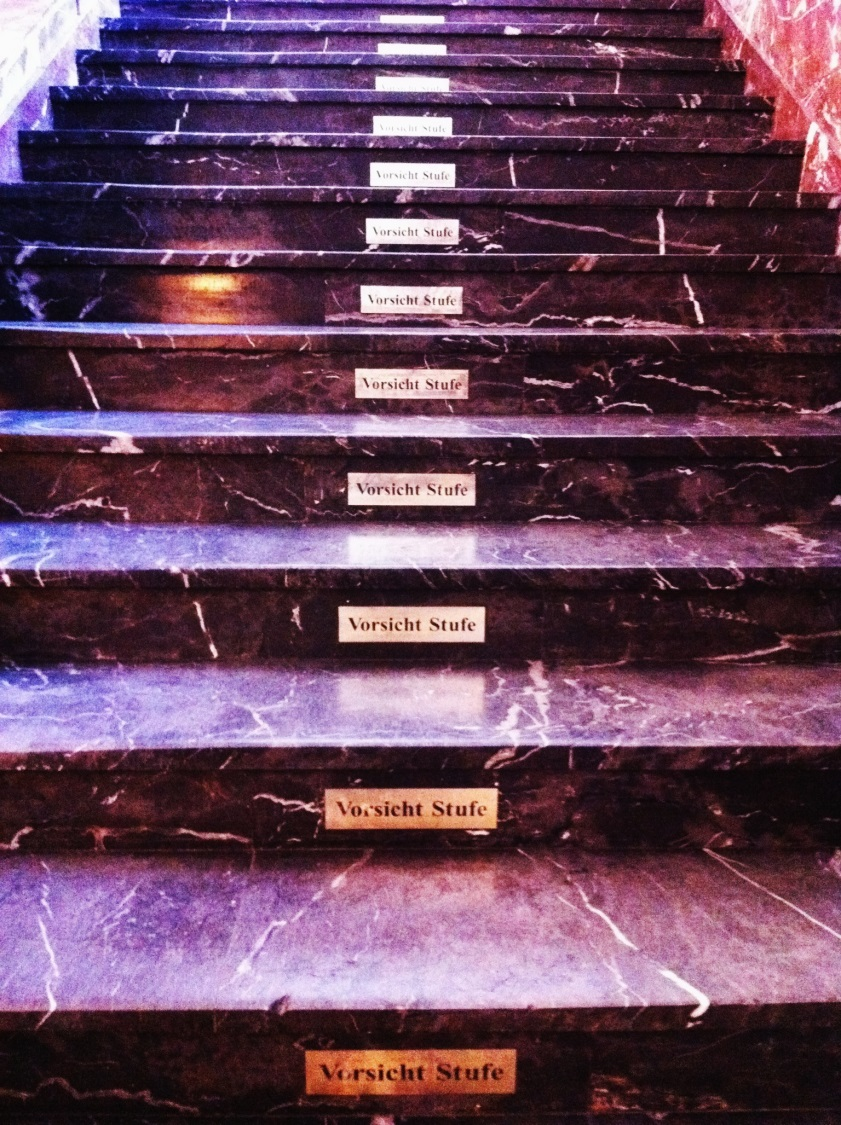
\includegraphics[width=\textwidth]{material/15Prag3}
\end{minipage}

\end{figure}

\end{frame}

%%%%%%%%%%%%%%%%%%%%%%%%%%%%%%%%%%%%%%%%%%%
\subsection{Übungen}
%%%%%%%%%%%%%%%%%%%%%%%%%%%%%%%%%%%%%%%%%%%
%% MyP: Contents
\iftoggle{sectoc}{
	\frame{
		%\begin{multicols}{2}
		\frametitle{~}
		\tableofcontents[currentsubsection,subsubsectionstyle=hide]
		%\end{multicols}
	}
}
%%%%%%%%%%%%%%%%%%%%%%%%%%%%%%%%%%%%%%%%%%%

\begin{frame}[shrink]
\frametitle{Übungen}

	\begin{enumerate}
		\item Gegeben sei der Satz unter (\ref{ex:08ue1}):
		
			\ea\label{ex:08ue1}
			Einige der US-amerikanischen Beamten wissen, wer Richard erdrosselt hat.
			\z
			\item [] Geben Sie bei jedem der Sätze unter (\ref{ex:08ue2})--(\ref{ex:08ue5}) an, ob es sich um eine Implikatur, oder ob es sich um eine Präsupposition zu (\ref{ex:08ue1}) handelt. Schreiben Sie die richtige Antwort hinter den jeweiligen Satz. Wenn es sich um eine Präsupposition handelt, testen Sie dies anhand eines der Präsuppositionstests. \\
		\textbf{NB:} Vorsicht, zuweilen wird keine der Relationen wiedergegeben!
		\ea\label{ex:08ue2} Es existieren US-amerikanische Beamte.
		\ex\label{ex:08ue3} Richard war ein Semantiker.
		\ex\label{ex:08ue4} Nicht alle US"=amerikanischen Beamten wissen, wer den Mord begangen hat.
		\ex\label{ex:08ue5} Richard wurde erdrosselt.
		\z	
	\end{enumerate}

\end{frame}

%%%%%%%%%%%%%%%%%%%%%%%%%%%%%%%%%%%%%%%%%%%

\begin{frame}
	\begin{enumerate}
		\item[2.] Bestimmen und kennzeichnen Sie zwei deiktische Ausdrücke im Satz (\ref{ex:08ue6}). Geben Sie zudem eine Anapher mit ihrem Antezendens an.
		\ea\label{ex:08ue6} Angelika hat gestern erwähnt, dass Irene sich dort mit den Formeln amüsiert hat.
		\z 
		\item[3.] Kreuzen Sie für Satz (\ref{ex:08ue7}) alle Sätze in der unten stehenden Liste an, die (konversationelle) Implikaturen dieses Satzes darstellen.
		\ea \label{ex:08ue7} Gottfried hat einige Nachbarn beleidigt.
		\z 
		\begin{itemize}
			\item[$\circ$] Gottfried hat einen Nachbarn.
			\item[$\circ$] Gottfried hat nicht alle Nachbarn beleidigt.
			\item[$\circ$] Gottfried ist ein unbeliebter Mensch.
			\item[$\circ$] Gottfried hat etwas Unhöfliches gesagt.
			\item[$\circ$] Gottfried hat einige Nachbarn nicht beleidigt.
		\end{itemize}
	\end{enumerate}
\end{frame}

%%%%%%%%%%%%%%%%%%%%%%%%%%%%%%%%%%%%%%%

\iftoggle{ue-loesung}{
	
	%%%%%%%%%%%%%%%%%%%%%%%%%%%%%%%%%%
%% UE 2 - 08 Pragmatik
%%%%%%%%%%%%%%%%%%%%%%%%%%%%%%%%%%

\begin{frame}
\frametitle{Übung -- Lösung}
	
	\begin{enumerate}
		\item Gegeben sei der Satz unter (\ref{ex:08ue1}):
		
	\begin{exe}
		\exr{ex:08ue1} Einige der US-amerikanischen Beamten wissen, wer Richard erdrosselt hat.
	\end{exe}

		\item [] Geben Sie bei jedem der Sätze unter (\ref{ex:08ue2})--(\ref{ex:08ue5}) an, ob es sich um eine Implikatur, oder ob es sich um eine Präsupposition zu (\ref{ex:08ue1}) handelt. Schreiben Sie die richtige Antwort hinter den jeweiligen Satz. Wenn es sich um eine Präsupposition handelt, testen Sie dies anhand eines der Präsuppositionstests. \\
		\textbf{NB:} Vorsicht, zuweilen wird keine der Relationen wiedergegeben!
	\begin{exe}
		\exr{ex:08ue2} Es existieren US-amerikanische Beamte. \textcolor{red}{\ras Präsupposition}
		\exr{ex:08ue3} Richard war ein Semantiker. \textcolor{red}{\ras weder noch}
		\exr{ex:08ue4} Nicht alle US"=amerikanischen Beamten wissen, wer den Mord begangen hat. \textcolor{red}{\ras Implikatur}
		\exr{ex:08ue5} Richard wurde erdrosselt. \textcolor{red}{\ras Präsupposition}
	\end{exe}

	\end{enumerate}
	
\end{frame}

%%%%%%%%%%%%%%%%%%%%%%%%%%%%%%%%%%%%%%%%%%%

\begin{frame}
	\frametitle{Übung -- Lösung}
	
	\begin{enumerate}
		\item[2.] Bestimmen und kennzeichnen Sie zwei deiktische Ausdrücke im Satz (\ref{ex:08ue6}). Geben Sie zudem eine Anapher mit ihrem Antezendens an.
	
	\begin{exe}
		\exr{ex:08ue6} Angelika hat gestern erwähnt, dass Irene sich dort mit den Formeln amüsiert hat.
	\end{exe}
		
		\begin{itemize}
			\item[] \textcolor{red}{Ausdruck: \emph{gestern}, Art: Temporaldeixis}
			\item[] \textcolor{red}{Ausdruck: \emph{dort}, Art: Lokaldeixis}
			\item[] \textcolor{red}{Anapher: \emph{sich}, Antezedens: \emph{Irene}}
			\item[] \textcolor{red}{Auch möglich: \emph{den Formeln} \ras Objektdeixis}
		\end{itemize}
		
	\end{enumerate}
	
\end{frame}

%%%%%%%%%%%%%%%%%%%%%%%%%%%%%%%%%%%%%%%%%%%%

\begin{frame}
	\frametitle{Übung -- Lösung}
	
	\begin{enumerate}
		\item[3.] Kreuzen Sie für Satz (\ref{ex:08ue7}) alle Sätze in der unten stehenden Liste an, die (konversationelle) Implikaturen dieses Satzes darstellen.
		
	\begin{exe}
		\exr{ex:08ue7} Gottfried hat einige Nachbarn beleidigt.
	\end{exe}

		\begin{itemize}
			\item[$\circ$] Gottfried hat einen Nachbarn.
			\item[\textcolor{red}{$\checkmark$}] \textcolor{red}{Gottfried hat nicht alle Nachbarn beleidigt.}
			\item[$\circ$] Gottfried ist ein unbeliebter Mensch.
			\item[\textcolor{red}{$\checkmark$}] \textcolor{red}{Gottfried hat etwas Unhöfliches gesagt.}
			\item[\textcolor{red}{$\checkmark$}] \textcolor{red}{Gottfried hat einige Nachbarn nicht beleidigt.}
		\end{itemize}
		
	\end{enumerate}


\end{frame}
	
}

%%%%%%%%%%%%%%%%%%%%%%%%%%%%%%%%%%%%%%%

